%--> Je Subsection Punkt Fragen formulieren.

%-------------------------------------------
% HEADER

% Roterfade der Einleitung:

% 1. Problem -> Kompatibilität
% 2. Ziel -> Lösung mit Übersetzungsprogramm
% 3. Abgrenzung Interpreter & Compiler -> Übersetzungsprogramm als Transpiler
% 4. Formale Grammatike -> Formale Grammatik als Vorrausetzung des Transpilers
% 5. JavaCC -> Implementierung der Formalen Grammtik mit JavaCC und damit des Transpilers

%-------------------------------------------

\section{Theoretische Grundlagen}
\subsection{Problemstellung}
	
Es gibt zwei grundlegende Probleme die eine PL/I zu Java Übersetzung lösen soll. 
Einerseits das Kompatibiltätsproblem von PL/I-Programmen, die auf modernen Platformen laufen sollen, wie etwa Cloud-Instanzen, oder Linux-Server. Andererseits die mit einem hohen Aufwand verbundene Wartung von bestehenden PL/I-Programmen. 
	
Bestehende PL/I Compilerlösungen führen aktuell zu einem Kompatibilitätsproblem. Der PL/I Compiler, der auf den meisten Computer-Systemen im Einsatz ist wird von IBM entwickelt und vermarktet. Hierbei handelt es sich um einen Compiler der expilziet für z/Os geschrieben wurde. Dabei ist z/Os ein Betriebssystem für die von IBM vermarkteten Großrechner. Eine kompilierung von PL/I auf einem herkömmlichen x86-Desktop Computer oder in der Cloud ist mit diesem Compiler nicht möglich. 
(https://www.ibm.com/de-de/products/pli-compiler-family) 

Eine Alternative bietet die Organisation GNU mit der GNU Compier Collection (GCC). Der Entwickler Henrick Sorensen entwickelte Teile des Frontends für einen PL/I Compiler. Dabei verwendete er das Backend, das die GCC zu verfügung stellt. Jedoch gab es bei diesem Projekt seit 2007 keine weiteren Neuerungen mehr. Der Entwickler gibt an, das bisher keine Zwischencode Erzeugung stattfindet, was diesen Compiler bisher unbrauchbar macht. Somit ist dieser Compiler keine Alternative zu dem von IBM.
(https://pl1gcc.sourceforge.net/) 

% @todo: Quellen
Heutzutage ist die gängige Möglichkeit, ein IBM 3270 Terminal zu emulieren, das eine Verbindung zum z/Os System herstellt, und den PL/I Code auf diesem zu kompilieren.
Weiterhin ist PL/I eine Altsprache, die seit den 1960er Jahren im Einsatz ist (IBM Quelle holen) und durch den Generationenwechsel an Entwicklern verliert. Wartung und Entwicklung werden so häufig schwer und teuer. (Quelle?)
(https://www.fruehes.berlin/wp-content/uploads/2011/02/PL-1-F-OS-360-V-4.0.pdf, erste Seite)

% @todo: Quelle
Java hingegen ist auf nahezu allen modernen Systemen durch die plattformunabhängige Java Virtual Machine (JVM) kompilierbar. 
(https://medium.com/@etherservices.vimalraj/can-i-run-java-programs-on-any-device-a-comprehensive-guide-31f736ca6ab1) (Oracle Quelle)

% @todo: Quelle
Insbesondere ist eine Kompilierung auch auf einem IBM-Großrechner mit z/Os möglich. (https://www.ibm.com/docs/en/zos-basic-skills?topic=zos-java)
Das macht Java zu einer flexibel Einsetzbaren Sprache. Weiterhin is Java die mit am meisten verwendete Programmiersprache in der heutigen Zeit. (Quelle?) Das führt zu einer höheren Anzahl an Entwickler, die in der Lage sind Java Programme zu warten.

% @todo: Begriffswahl
% Was ist ein Transpiler?
Um nun Java für die Lösung der dargelegten Probleme zu verwenden, wird ein Programm benötigt, welches PL/I Quellcode in Java Quellcode übersetzt. Ein solcher Transpiler verarbeitet PL/I-Code so, dass aus diesem Java-Code generiert werden kann. Dabei ist es möglich das der Entwickler, selbst wählt wie er welche Ausdrücke übersetzt. Ist der Programmcode erstmal in Java übersetzt worden, kann dies durch die JVM kompiliert werden.

Am Ende ist zwar der Quellcode übersetzt und auch kompilierbar, jedoch ist erst ab diesem Punkt erst die tatsächliche Qualität des Programms zu erkennen. Faktoren wie Lesebarkeit und Erweiterbarkeit des übersetzen Programmcodes gehen in die Beurteilung mit ein. 
Die Beurteilung der Qualität des Programms ist auch von Zielaspekten der Benutzer abhängig. Für das zu entwickelnde Übersetzunsgporgramm, wurden Zielgruppen definiert die im nachfolgenden Kapitel 1.2 weiter erläutert werden sollen. Diese Zielgruppen sind für weitere Gestaltungsentscheidungen in der Entwicklung des Programms wichtig.

%Anderseits auch die veränderte Laufzeit-Performance. Die Laufzeit-Performance kann durch eine Übersetzung verschlechtert, wie auch verbessert werden. Somit ist nicht nur die reine Übersetzung Teil der Problemstellung, sondern es gilt auch die Übersetzung zu beurteilen. 
\pagebreak
     
% %todo: Cross Compiler? - Hat hier eig nix zu suchen, ist Thema für Boostrapping aber nicht für Transpiler
     
     
     
% 	 Welches Problem löst das Programm?
%	 Probleme 
%			 1. Nicht auf jedem System läuft PL/I, besonders nicht auf modernen x86 bzw. Cloud.
%			 2. PL/I ist eine weniger verwendete Sprache, Wartung teuer &  Schwer.

%	 (Hinführung zum Problem:
%	 Historisches Kompatibilitätsproblem -> Nicht auf jedem System lief jede Assambler Sprache, Problem: hoher Aufwand und Unflexibel
% 	 Deshalb -> Compiler mit Hochsprache, der Code für das Backend des Compilers, bspw. C's Gcc Compiler
%    in Assambler Sprache des Systems übersetzt.)? **Hier einen Cross Compiler erklären bzw. im Zusammenhang mit dem Historischen Problem.**

%	 Problem mit PL/I -> Pl/I Compiler rar bzw. nur für Großrechner Systeme vorhanden   
%	 Es gibt zwar einen GCC Pl/I Compiler, dieser wird aber seit 2007 nicht mehr weiterentwickelt. Eine Weiterentwiclung könnte auch Interessant %    sein, löst aber nicht das Problem der teuren Wartung von Programmen in PL/I.

% 	 
%	 Lösungsvorschlag zu 1 -> PL/I zu Java Transpiler bauen Java und JVM relativ System unabhängig und damit Ideale Zielsprache für eine 
%	 hohe Kompatibiltätsrate.Um zum Beispiel Pl/I Programm die auf einem Großrechner laufen auch auf einem x86 On-Prem Server oder einer Cloud
%    zu betreiben. **Hier die Frage klären was ein Transpiler ist**
%	 
%    Lösungsvorschlag zu 2 -> Java ist den großteil der Softwareentwickler bekannt und eine Wartung ist leichter.
%
    
\subsection{Zielsetzung}
% Herleitung von der Problemstellung	
Das Ziel dieser Arbeit leitet sich aus der eingeführten Problemstellung in Kapitel 1.1 ab. Allgemein soll ein plattformunabhängiges Programm entstehen, dass die  Entwicklung und Transformation von Pl/I Programmen ermöglicht. Die zugrundeliegende Arbeit stellt die Entwicklung, sowie die Gestaltung der Software dar und wird schlussendlich diskutiert. 

% @todo: Referenz zu Begriffsklärungsabsatz
% Zielgruppen Zusammengefasst	
Somit richtet sich diese Arbeit und der Transpiler teils an juniore Entwickler für Anwendungen in den Sprachen PL/I bzw. Java. Für diese Nutzergruppe soll der Transpiler ein Hilfswerkzeug darstellen. Eine andere Nutzergruppe sind Administratoren, die den Transpiler selbst anpassen und erweitern möchten. Ermöglicht wird dies durch eine modulare Architektur. 
	
% Junior Entwickler die gerade in PL/1 einsteigen.
Juniore Entwickler profitieren von dieser Arbeit als Einstiegspunkt in die Programmiersprache PL/I. Dadurch das es schwierig ist ein PL/I-Progamm auf einem herkömmlichen Desktop Computer zu kompilieren, soll das erarbeite Programm Abhilfe schaffen. Beispielhaft könnten Entwickler den Transpiler als Test-Umgebung für eigen entwicklete PL/I-Programme benutzen.

% Lernhilfe
Für Entwickler, die mehr Erfahrung mit Java haben, eignet sich das Übersetzungsprogramm als Lernhilfe. Es wird ihnen so erleichtert, PL/I-Programme zu analysieren. Sie können bestehende Kenntnisse in Java anwenden, um gleiche Muster in PL/I wiederzuerkennen. Dies kann den Lernprozess beschleunigen. In dieser Arbeit wird dabei die Gestaltung von Übersetzungsmustern, des zugrundeliegenden Programmes diskutiert. Hierzu wird an Vor- und Nachteile gewählter Gestaltungen herangeführt.

% Online-Smoketest von PL/I Code -> %todo: Verschieben nach Erweiterbarkeit (Schlusskapitel), weil momentan noch nicht vollständige Grammatik realisiert.
Ein weiterer denkbarer Einsatzbereich ist es, den PL/I-Code auf seine Richtigkeit zu testen. Wird mithilfe des Programms erfolgreich das PL/I-Programm in Java übersetzt, so sollte auch ein herkömmlicher PL/I-Compiler auf einem Mainframe den Code ausführen können. Somit eignet sich das Programm auch für Smoke-tests von Anwendungen.

% Benutzbarkeit
Der Übersetzer aus der Projektarbeit-IV konnte bisher über die Kommandozeile, sowie der IDE Eclipse verwendet werden. Diese ursprüngliche Benutzung des Programms führte zu einer erhöhten Fehleranfälligkeit und Dokumentationsbedarf. Ein vereinfachtes Darstellungskonzept, welches in Kapitel 2.? Vorgestellt wird, bietet den Benutzern einen leichteren Einstieg in das Programm.
Die Komplexität der Benutzung wird durch ein Graphical-User-Inferface (GUI) vereinfacht. Das Konzept dieser GUI soll dem eines Übersetzers der natürlichen Sprache, wie etwa 'DeepL' oder 'Google-Translate', ähneln. Mit diesen Konzepten sind Juniore Entwickler vertraut, erleichtert den Einstieg in die Programmiersprache PL/I, das Testen des PL/I Codes, sowie die schnelle Übersetzung.

%  Entwickler die das Programm eigenständig erweitern, verändern wollen.
Durch die modularisierte Gestaltung des Übersetzers können Administratoren selbst Module austauschen und erweitern, etwa durch eine API-Schnittstelle zu externen Übersetzungsbibliotheken/-services. 

%  Zusammenfassung und hinführung zum nächsten zu dem Unterschied Interpreter und Compiler
Auch wenn beide Zielgruppen unterschiedliche Ausprägung der Zielvorstellung haben, wollen beide eine Übersetzung von einer Quellsprache in eine Zielsprache erreichen. Die Art und Weise des Transpiler sind dabei unterschiedlich. Ein Übersetzungsprogramm kann sowohl als Interpreter und als Compiler gestaltet werden. In dem nachfolgenden Kapitel 1.3 werden die Begriffe voneinander abgegrenzt. 
	
% Aufteilung der Zielstellung:
% 1. Allgemein; Ableitung aus der Problemstellung
% 2. Zielgruppen spezfifisch
% 2.1 Einfache und unkomplizierte Lösung
%
% 2.2 Erweiterung des Transpilers bzw. ersetzen von Modulen	
	
% - Wie eine Art JavaScript Minifier oder 
%  Wer ist die Zielgruppe?
%  - Junior Entwickler die gerade in PL/1 einsteigen.
%   - Lernhilfe
%  - Online-Smoketest von PL/I Code
%   - Benutzbarkeit
%   - Entwickler die das Programm eigenständig erweitern, verändern wollen.
 
%  Ziele der Architektur (Zielgruppe Entwickler)
%  - Perspektive des Entwicklers
%  - Perspektive des Benutzers
    \pagebreak

\subsection{Abgrenzung Interpreter und Compiler}
% Wie können Programme ausgeführt werden?
Nachdem die Zielsetzung klar ist, untersucht dieses Kapitel die Unterschiede zwischen Compilern und Interpretern genauer.
  
% Wie arbeitet ein Compiler?
Ein Compiler besteht aus einem Frontend und einem Backend. Das Frontend umfasst die lexikalische Analyse, die syntaktische Analyse, die semantische Analyse und die Symboltabelle, die in jedem dieser Schritte verwendet wird. 
Das Ergebnis des Frontends ist eine Zwischencodedarstellung. Diese Zwischencodedarstellung wird an das Backend übergeben, um daraus Maschinencode zu generieren. Der Maschinencode kann dann auf dem zugrundeliegenden System ausgeführt werden. (Compilers: Prinicples and Techniques, S. 106ff.)
\pagebreak
% @todo: Hier evtl. Abbildung...
\begin{figure}[h]
  \centering
  \caption{Funktionsweise eines Compilers}
  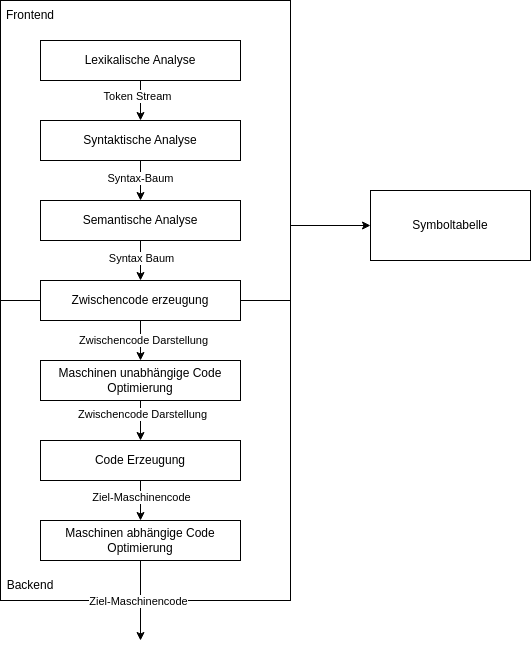
\includegraphics[scale=0.75]{compiler-ablauf-diagramm.png}
  \label{fig:compiler}
\end{figure}
\pagebreak
Abbildung ?.? zeigt eine Übersicht und das Ergebnis der einzelnen Phasen. Die Abbildung unterteilt den Ablauf wie eingangs beschrieben in Frontend und Backend.

In der ersten Phase teilt der Compiler den eingegebenen String in Tokens auf. Danach entsteht ein Syntaxbaum, der in eine Zwischencodedarstellung umgewandelt wird. Ab diesem Punkt beginnt das Backend des Compilers. Zuerst erzeugt es maschinenunabhängigen Code und anschließend maschinenabhängigen Code. Dieser maschinenabhängige Code ist auf dem zugrundeliegenden System ausführbar. (Compilers: Principles and Techniques, s. 30) 
Abbildung ?.? zeigt die Allgemeinen Phasen eines vollumfänglichen Compilers. 

%  Warum ein Transpiler?
Ein Compiler kann auf verschiedene Weise implementiert werden, wobei die Ausprägung der Prozessschritte, wie beispielsweise das Ergebnis der syntaktischen Analyse, häufig variiert. Ein One-Pass-Compiler erzeugt keinen Zwischencode, sondern führt den Code direkt aus. Diese Methode wurde ursprünglich angewendet, um Speicherplatz zu sparen, da frühe Computer nur begrenzte Kapazitäten hatten und keine Zwischenergebnisse speichern konnten. Ein Beispiel für eine Sprache, die mit einem One-Pass-Compiler kompiliert wird, ist Turbo Pascal. (https://keleshev.com/one-pass-compiler-primer)

Ein Source-to-Source-Compiler unterscheidet sich von einem herkömmlichen Compiler durch die Zielsprachen, in die er übersetzt. Während ein C-Compiler den C-Code nach der Zwischencodeerzeugung in Assemblersprache und anschließend in Maschinencode übersetzt, wandelt ein Source-to-Source-Compiler beispielsweise C-Code in Java-Code um. Der Java-Code wird dann in den Bytecode des Java-Compilers übersetzt und schließlich mithilfe der JVM kompiliert. Ein weiteres Synonym für ein solches Programm ist "Transpiler". Abbildung ?.? illustriert die Arbeitsweise eines solchen Transpilers.
\pagebreak
\begin{figure}[h]
  \centering
  \caption{Funktionsweise eines Transpilers}
  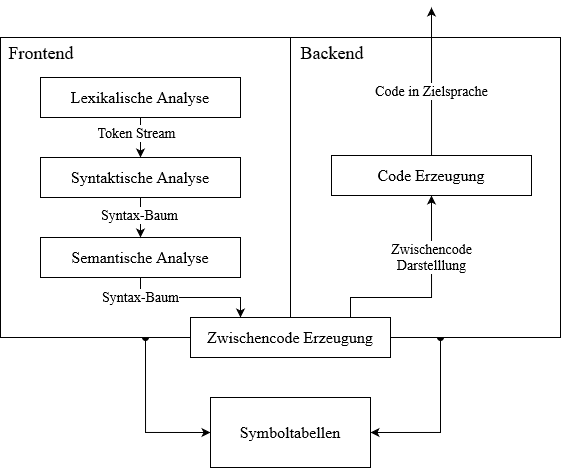
\includegraphics[scale=0.75]{transpiler-diagramm.png}
  \label{fig:transpiler}
\end{figure}
\pagebreak
Ein Vergleich von Abbildung ?.? mit Abbildung ?.? zeigt, dass die ersten Phasen bis zur Zwischencodeerzeugung gleich bleiben. In Abbildung ?.? sind jedoch die Prozesse des Frontends neben denen des Backends dargestellt, um die Sprachebene zu verdeutlichen.

Ein Compiler übersetzt den Eingabecode in eine maschinennahe Programmiersprache wie Assembler. Ein Transpiler hingegen behält die Sprachebene der Eingabesprache bei, was die nebeneinanderliegende Darstellung erklärt. In Abbildung ?.? werden zudem die Phasen des Backends reduziert, da keine Übersetzung in eine maschinenabhängige Sprache erforderlich ist. Anschließend folgen die Prozesse des Compilers aus Abbildung ?.? da auch das Programm der Zielsprache kompiliert werden muss.


Sowohl One-Pass-Compiler, Transpiler als auch herkömmliche Compiler übersetzen das Programm basierend auf seiner Gesamtstruktur. (https://keleshev.com/compiling-to-assembly-from-scratch/excerpt-compiling-to-assembly-from-scratch.pdf)[S. 18ff.] Eine alternative Konzeptionsart wird durch den Interpreter dargestellt.


% Wie arbeitet ein Interpreter?
Im Vergleich zu einem Compiler hat der Interpreter weder ein Frontend noch ein Backend. Bei der Verwendung eines Interpreters wird der Quellcode direkt ausgeführt. Es gibt keine klare Trennung zwischen einem Frontend, das eine unabhängige Repräsentation des Codes erzeugt, und einem Backend, das diese Repräsentation interpretiert. Zusammengefasst wird das Programm nicht erst in eine Zielsprache übersetzt, sondern direkt ausgeführt.

Programmiersprachen, die von einem Interpreter ausgeführt werden, sind beispielsweise PHP3, Ruby, JavaScript und Shell. Es ist auch möglich, sowohl einen Interpreter als auch einen Compiler für die Interpretation einer Sprache zu verwenden. Die Sprache 'Go' beispielsweise nutzt sowohl einen Compiler als auch einen Interpreter. Dabei wird das Go-Programm mit dem Befehl \verb+go build+ kompiliert und mit \verb+go run+ sofort durch den Interpreter ausgeführt. (https://craftinginterpreters.com/a-map-of-the-territory.html)
Um die Funktionsweise eines Interpreters nachzuvollziehen, soll die Skriptsprache Shell näher betrachtet werden. Shell wird auf den meisten Unix-ähnlichen Betriebssystemen eingesetzt.
  
% Absatz: Ein Interpreter am Beispiel von Bash
Auf unixoiden Betriebssystemen dient die Shell als Interpreter für Skriptprogramme. Sie nimmt Benutzerbefehle direkt oder aus Skriptdateien entgegen und übergibt sie zur Ausführung an das Betriebssystem. Außerdem übernimmt sie die Ausgabesteuerung und kontrolliert die Datenströme. 

% @todo: Was unterscheidet die Shell von einem Übersetzer(Compiler)
(https://en.wikipedia.org/wiki/Listofcommand-lineinterpreters)

Abbildung 1.1 stellt den Ablauf der Skript-Interpretation dar.
\begin{figure}[h]
  \centering
  \caption{Ablauf der Interpretation eines Shell Programms}
  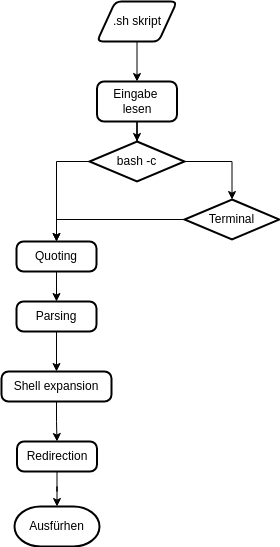
\includegraphics[scale=0.75]{shell_interpreter.png}
  \label{fig:shell}
\end{figure}
\pagebreak

Abbildung 1.1 zeigt den Ablauf eines Shell-Skripts, beginnend mit der Eingabe des Skripts von oben. Neben Shell-Befehlen, die auch in einer Befehlszeilenumgebung ausgeführt werden können, kann das Shell-Skript auch Verzweigungen und Schleifen enthalten.

Die Eingabe des Shell-Skripts wird zeilenweise gelesen, entweder über ein Terminal oder durch den Befehl \verb+bash -c+. Beide Eingabemethoden führen zur ersten Phase des Shell-Interpreters.

Die Phase des Quoting folgt dem Prinzip der lexikalischen Analyse, bei der alle Sonderzeichen entfernt werden, wie zum Beispiel Kommentare oder Backslashes. Sobald das Quoting abgeschlossen ist, entsteht ein String, der nur aus den Tokens eines Ausdrucks besteht.

Anschließend beginnt das Parsing, das der syntaktischen Analyse im Kompilierprozess ähnelt, jedoch keine Zwischencodeerzeugung beinhaltet. Hier wird lediglich zwischen einfachen Befehlen und zusammengesetzten Befehlen unterschieden. Einfache Befehle umfassen das Ausführen der integrierten Shell-Programme wie \verb+ls+, \verb+wc+ oder \verb+mkdir+. Zusammengesetzte Befehle bringen zusätzliche Logik in das Shell-Programm ein, wie zum Beispiel \verb+if+, \verb+while+ oder \verb+case+.

Der Übersetzungsprozess setzt sich mit der Shell-Expansion fort, bei der in einem Befehl eingebettete relative Ausdrücke durch ihre absoluten Repräsentationen ersetzt werden. Zum Beispiel würde im Ausdruck \verb+echo ${pwd}+ das \verb+$pwd+ durch den absoluten Pfad des aktuellen Verzeichnisses ersetzt.

Schließlich wird die Ausgabe des Shell-Skripts über die \verb+stdio+-Bibliothek ausgegeben.
(https://www.gnu.org/software/bash/manual/bash.html#Shell-Operation)

In diesem gesamten Prozess wird ausschließlich die Shell-Skriptsprache verwendet. Der Quellcode wird nicht von einer Hochsprache in eine Niedrigsprache oder eine andere Hochsprache umgewandelt. Dies verdeutlicht einen zentralen Unterschied zwischen einem Interpreter und einem Compiler: Es entsteht keine Repräsentation des Codes in einer anderen Sprache. Vom Eingang des Codes bis zum Ergebnis des Programms bleibt der Interpreter bei einer Sprache.

% Absatz: Zusammenfassende Unterscheidung zwischen Interpreter und Transpiler, Was sind gemeinsamkeiten und unterschiede von Transpiler und interpreter?

Zusammenfassend zeigen sich sowohl Ähnlichkeiten als auch Unterschiede zwischen einem Interpreter und einem Compiler. Beide durchlaufen die Phasen der lexikalischen und syntaktischen Analyse, wobei sie den Quellcode zunächst bereinigen, um Kommentare, Leerstellen oder andere für die Übersetzung irrelevante Symbole zu entfernen. Anschließend erfolgt entweder die direkte Übersetzung des Quellcodes oder die Erzeugung einer unabhängigen Repräsentation.

Der entscheidende Unterschied liegt darin, dass der Interpreter den Quellcode lediglich zeilenweise direkt übersetzt, während der Compiler das Programm in eine andere Form transformiert und liest. Dabei stehen die verwendeten Ausdrücke des Eingabecodes in Beziehung zueinander, beispielsweise durch die Verschachtelung von Verzweigungen und Schleifen.

Um PL/I-Code korrekt in Java zu übersetzen, sind Verbindungen zwischen den Ausdrücken wichtig. Eine bloße zeilenweise Übersetzung könnte zu einem Java-Programm führen, das kaum objektorientierte Paradigmen enthält. Daher wird in dieser Arbeit gegen einen Interpreter entschieden, da das Zielprogramm solche Elemente enthalten soll.

 Wie bereits in Abbildung ?.? dargestellt, übersetzt ein Transpiler eine Hochsprache in eine andere. Da das Programm die Programmiersprache PL/I in eine andere Programmiersprache, wie in diesem Fall Java, übersetzen soll, ist die Konzeptionsweise eines Transpiler ideal.

Um die zugrunde liegende Sprache PL/I korrekt zu verarbeiten, bedarf es eines Transpilers einer Grammatik. Das folgende Kapitel wird Grammatiken formaler Sprachen wie PL/I und Java genauer beleuchten.

% - Erweiterung des Umfangs während der Laufzeit
% - Trennung Laufzeit/Konzeptionsphase

% - Hier erwähnen das eine geminsamkeit die definition von Grammatiken ist, dann überleiten zu Formale Grammatiken.
% - Auch Entscheidung treffen was genau der Transpiler ist, Compiler oder Interpreter
\pagebreak
   
   
\subsection{Formale Sprachen und ihre Grammatiken}
% Warum braucht ein Compiler eine Grammatik?
In dem vorangegangen Kapitel wurden unterschiedliche Formen der Sprachinterpretation eines Computers vorgestellt. Damit die Interpretation von Sprachen korrekt erfolgt, braucht ein Computer Regeln. Grammatiken beinhalten diese Regeln. Damit der Transpiler korrekt arbeitet wird eine definierte Grammatik benötigt. Nur so können die Prozessschritte der Lexikalischen- und der Syntatkischen Analyse korrekt erfolgen. Denn diese Schritte prüfen den eingegeben Quellcode auf seine grammartikalische Richtigkeit. Bevor also die Sprachliche Analyse erfolgen kann, sollte eine Grammatik angwendet werden.
	
% Woraus besteht eine Grammatik?
Um eine Grammatik anzuwenden muss klar sein, um welche Grammatik es sich handelt. Weiterhin sollte bestimmt werden welche Art von Sprache beschrieben werden soll. 
Da es sich bei einem Transpiler um ein Computeprogramm handelt, ist die behandelende Sprache eine fromale Sprache. Eine formale Sprache unterscheidet sich von einer natürlichen Sprache in der Anwendungsform. Die Anwendung von solchen Sprachen dient der logisch präzisen Beschreibung von Ausdrücken. (introduction to formal languages and automata, S. 149ff.) Eine Grammatik besteht aus Variablen, Terminalsymbolen, einen Startsymbol und einer Produktion. Zusammengefasst in:

\begin{center}
\begin{equation}
G=(V,T,S,P)
\end{equation}
\end{center}

Hierbei \verb+V+ für Variablen bzw. Nicht-Terminalsymbole, \verb+T+ für Terminale, \verb+S+ für Start und \verb+P+ für Produktion steht. Dabei ist \verb+S+ ein Teil von \verb+V+. (introduction to formal languages and automata, S. 31ff.)


% Welche Typen von Grammatiken gibt es? Chomsky Hierarchie
Grammatiken lassen sich weiter durch die Chomsky Hierarchie spezifizieren. Noam Chomsky unterteilt Grammatiken in vier Ebenen. Ebene null beschreibt unbeschränkte-, Ebene eins kontextsensitve-, Ebene zwei kontextfreie- und Ebene drei reguläre Grammatiken.(https://hpi.de/friedrich/teaching/units/grammatiken.html) 

\pagebreak

Wobei unbeschränkte Grammatiken immer gegeben sind, solange mit einer Produktion auch mindestens ein Nicht-Terminalsymbol beschrieben wird. Das ist bei Grammatiken von Programmiersprachen der Fall. Denn bei der Variablen-Deklaration in der Programmiersprache PL/I entsteht folgende Produktion:

% @todo: PL/I Verwenden und Kontext herstellen
\begin{center}
\begin{equation}
S \to \mathbf{if}\: expr\: \mathbf{then}\: stmt\: \mathbf{else}\: stmt\: | \mathbf{if}\: expr\: \mathbf{then}\: stmt;
\end{equation}
\begin{equation}
expr \to expr\: op\: term\: | term
\end{equation}
\begin{equation}
op \to \mathbf{>}\: |\: \mathbf{<}\: |\: \mathbf{=}\: |\: \mathbf{!}
\end{equation}
\begin{equation}
term \to term\: multOp\: factor\:
\end{equation}
\begin{equation}
factor \to \mathbf{id}\: |\: \mathbf{constant} 
\end{equation}
\end{center}
 
Mit der beschriebenen Grammatik ist folgender Ausdruck zulässig.

\begin{verbatim}
IF A > B THEN 
	CALL proc_1;
ELSE 
	CALL proc_2;
END
\end{verbatim}

Nicht zulässig ist hingegen.

\begin{verbatim} 
CALL IF THEN A > B proc_1;
\end{verbatim}

% @todo: Keine Hierachie Einordnung, ledilgich nennen das es sie gibt.
% @todo: Beispiel-Parsebaum analyse, https://en.wikipedia.org/wiki/LR_parser 
Somit ist die Grammatik einer Programmiersprache kontextsensitiv. 
Bei einer Verzweigung in PL/I ist es eindeutig das der Kontext der Terminalsymbole zu den Nicht-Terminalsymbolen zu berrücksichtigen ist. Jedoch kann auch eine mehrdeutigkeit entstehen. Zusätzlich sollte deshalb auf der linken Seite genau ein Nicht-Terminalsymbol stehen. Somit ist die definierte Grammatik ebenfalls Kontextfrei. 
Weiterhin kann in diesem Beispiel die Produktion als Terminalfolge aufgebaut werden. Etwa mit: 

\begin{center}
\begin{equation}
S \to TB \to int | double | float B \to AD \to A...Z|a...z D \to 0...9|D;
\end{equation}
\end{center}

% @todo: Nochmal überprüfen ob das stimmt.
Jedoch ist dieser Ausdruck damit nicht Regulär. Durch den Rekursiven Aufruf am Ende kann kein endlicher Automat erzeugt werden. Die Grammatik bleibt also höchstens von Typ 2.
	
% Wie werden Grammtiken in einem Transpiler Programm verwendet?
Die bisher definierten Grammatiken sind in dem Sinne von Bedeutung, weil die Lexikalsiche und Syntaktische Analyse des Transpilers aus einer solchen Grammatik erzeugt werden. Mithilfe einer Grammatik wird ein Parser definiert aus durch den Compiler-Compiler JavaCC erzeugt wird. 
Für den PL/I-Transpiler bedeutet, dass die aktuelle PL/I-Grammatik für den Parser definiert werden muss. Die aktuellste Grammatik wird durch IBM, in der PL/I Language Referenz definiert. Aus dieser wird mithilfe von JavaCC ein Parser erzeugt. Weshalb in dem folgenden Kapitel 1.5 der Compiler-Compiler und die dazugehörige Grammatik näher beschrieben wird.

% - Theoretischer Abriss
% - Einordnung der resultate der PA 4
%- PL/1 Syntax Wo zu finden? Welche Version der Sprache? 
%	- Reguläre Ausdrücke Syntax, Beispiel einer Grammatik die ich mit verwende, Typ einer Grammatik
%  - Literatur
%    - Chomsky Hierarchie Bücher
%    - https://www-igm.univ-mlv.fr/~berstel/LivreCodes/Codes.html
%  - Woraus besteht eine Grammatik?
%   - Wie lassen sich Grammatiken der Komplexität nach anordnen?
%  - Chomsky Hierarchie
%  Erst Chomsky Hierachier, dann nach Komplexität einordnen und am Beispiel von Regulären Ausdrücken und PL/I Grammatik einführen.
     
\subsection{Anwendung von Formalen Grammatiken in JavaCC}
% 1. Was ist ein Compiler-Compiler? (Verbindung von formalen Grammatiken zu JavaCC)

Der Lexer der die lexikalische Analyse und der Parser, der die Syntaktische Analyse durchführt werden durch JavaCC erzeugt. 
JavaCC ist ein Compiler-Compiler der aus einer formalen Grammatik einen Lexer und einen Parser generiert. 
In Kapitel 1.3 wurde bereits in die Thematik der formalen Grammatiken eingeführt, in diesem Kapitel wird nun die praktische implementation dieser Grammatiken im Zusammenhang mit dem Transpiler beschrieben.

Ein Compiler-Compiler ist eine Technologie mit der aus einer formalen Beschreibung einer Grammatik ein Lexer und ein Parser erzeugt werden. 
Der Lexer und der Parser wenden die in der Grammatik definierten Regeln an und verarbeiten entsprechend die übergebenen Ausdrücke.
Die Darstellung der Grammatik erfolgt in der Regeln in einer Art erweiterten Backus-Naur-Form (EBNF). 
Beispielhafte Compiler-Compiler sind neben JavaCC, Yacc, Antlr und Lexer.
In Kapitel 1.3 wurde bereits vereinfacht eine Produktion aus der PL/I-Grammatik dargestellt. Ähnlich erfolgt auch die Darstellung in einer Grammatikdatei. Folgendes Beispiel zeigt die Darstellung eines \verb+IF ELSE+ Ausdrucks. 
(https://javacc.github.io/javacc/)

\begin{verbatim}
void if_statement() #IF :
{}
{
  < IF > bool_expression() (bool_operation() bool_expression() )*
  < THEN >proc_body()
  [< ELSE >
  	proc_body()]
  	
}
\end{verbatim}

In JavaCC besteht die Möglichkeit die Beschreibung von Produktionen in Methoden zu Kapseln.
In Zeile 1 ist der Methodenkopf zu sehen. In diesem Fall erzeugt die Methode \verb+if_statement+ keinen Rückgabwert.
Das durch die Raute gekennzeichnete Symbol ist die Repräsentation im Parsebaum und zusätzlich auch die Darstellung im Zwischencode.
Im Körper der Methode wird der If-Ausdruck weiter definiert. Terminalsymbole werden in der JavaCC Grammatik mit den größer-als und kleiner-als Zeichne umrandet. Die Nicht-Terminalsymbole hingegen sind wie im Listing ?.? dargestellt weitere Methoden, die wiederum weitere Ausdrücke beschreiben.
Ähnlich wie bei der Produktion aus 1.3, so lange bis lediglich Terminalsymbole übrig bleiben.
Die Methode \verb+bool_expression+ etwa, beschreibt einen zulässigen Boolschen Ausdruck, der durch einen weiteren boolschen Operator mit einem weiteren booleschen Ausdruck verknüft werden kann.
Letzter Ausdruck, kann Leer sein und beliebig of wiederholt werden. Das ermöglich komplexe boolsche Operationen.

Weiterhin wird in der Methode \verb+proc_body+ beschrieben welche Ausdrücke in dem Verzweigungskörper zulässig sind. Dazu zählt bspw. auch eine weitere \verb+IF ELSE+ Verzweigung. So werden auch verschachtelte Ausdrücke möglich.
Werden nach und nach die Methoden durch den Compiler-Compiler aufgerufen, ergibt sich eine Regel für Verzweiguns-Ausdrücke. Nach diesem Prinzip ist die gesamte Grammatik gestaltet. 
Die Wurzel aller Methoden, die einen Ausdruck beschreiben, ist debei die Wurzel Methode \verb+program+, welche das gesamte Programm darstellt. Eine solche Kapselung macht die Grammatik übersichtlich.
Aus dem definierten Ausdruck aus Listing ?? wird schlussendlich ein Parsebaum erzeugt, der durch die folgenden Module weiter verarbeitet wird.

% Warum ein Compiler-Compiler verwenden?

Ein Compiler-Compiler generiert somit einen fertigen Parser, aus einer Datei in der eine Grammatik beschrieben wird. Nun gibt es auch die Möglichkeit einen Parser und Lexer selbst zu programmieren. In der Version aus der Projektarbeit-4 wurde ursprünglich ein selbstgeschriebener Lexer verwendet.
Jedoch birgt dieses Vorgehen einen Nachteil. Die Grammatik für den Transpiler ist an zwei stellen definiert und muss somit auch an zwei Stellen gewartet werden.
Wird in die Grammatikdatei für den Parser ein neuer Ausdruck hinzugefügt, muss dieser Ausdruck auch durch den Lexer verarbeitet werden können.
Ursprünglich musste so der Lexer angepasst werden und die Grammatikdatei für den Parser. 
Das führte zu einem erhöhten Arbeitsaufwand und Fehleranfälligkeit. Schlussendlich wurde der selbstgeschriebene Lexer entfernt und der von JavaCC definierte Lexer verwendet.
Somit ist ein Compiler-Compiler gut dazu geeignet den Arbeitsaufwand für die Entwicklung eines Compilers, bzw. eines Transpilers zu reduzieren. 
Es lohnt sich auch bei der Entwicklung auf bereits definierte Resourcen zurückzugreifen. 
Grammatiken für Cobol und Java wurden bereits von der JavaCC Community bereitgestellt. (https://javacc.github.io/javacc/)
Im Fall von PL/I ist keine Grammatik vorhanden. Weshalb bei der Entwicklung des Transpilers, die IBM Language Reference für PL/I die Hauptquelle für die Grammatikdatei ist.  
Verkürzt beschrieben, wird auf den Compiler-Compiler JavaCC zurückgegriffen um den Arbeitsaufwand der Entwicklung zu reduzieren. 

% @todo Wie funktioniert JavaCC ? Wie kann JavaCC die formale Beschreibung umsetzen ? (Erzeugung eines Parsers beschreiben)
Der Arbeitsaufwand wird eben durch die automatisierte Arbeitsweise des Compiler-Compilers ermöglicht. Bei diesem Prozess werden verschiedenste Java Klassen erzeugt. Für den PL/1-Transpiler werden nachfolgende Klassen erzeugt.

% @todo: Beschreibung hinzufügen
\begin{tabular}[h]{l|c|r}
Klasse & Beschreibung \\
\hline
JJTPl1ParserState.java & ... \\
Node.java & ... \\
ParseException.java & ... \\
Pl1Parser.java & ... \\
Pl1ParserConstant.java & ... \\
Pl1ParserTokenManager.java & ... \\
Pl1ParserTreeConstants.java & ... \\
SimpleCharStream.java & ... \\
SimpleNode.java & ... \\
Token.java & ... \\
TokenMgrError.java & ... \\
parser.jjt & ... \\
\end{tabular}


JavaCC generiert dynamisch den eigentlichen Parser, hier Pl1Parser, den TokenManager und die ParserConstants Klasse. Die restlichen Klassen sind Boilerplate-Code und werden bei jeder Grammatik generiert. Diese werden auch nur beim initalen kompilieren generiert.

% Wie wird JavaCC in die Entwicklung des Transpiler eingebunden ? (Hinleitung zur Architektur beschreibung)
Durch die Verwendung des JavaCC Jjtree-Moduls, kann global innerhalb des Projekts auf den Parse-Baum zugegriffen werden. 
Es werden zusätzlich die für den Parsebaum benötigten Klassen, \verb+Node+ und \verb+SimpleNode+ erzeugt.
Der Prase-Baum wird unteranderem durch die Module verwendet, die die Semantische-Analyse und -Synthese repräsentieren.
Erst durch diese wird der Java-Code erzeugt.
Ebenfalls wird für den Parser ein File-Stream benötigt, ein Scanner liefert solchen.
Neben den Parser werden also weitere Module verwendet um schlussendlich den Java-Code für den Benutzer bereitzustellen.
Die gesamte Architektur des Transpilers und dessen weitere Module wird in dem nachfolgenden Kapitel betrachtet. 
Hier werden auch die Technologien vorgestellt die neben JavaCC verwendet werden. 

\section{Technisches Vorgehen}
\subsection{Techstack}
Um den Transpiler weiter zu entwickeln sind Schritte notwendig die, die Qualität des bestehenden Projektes erhöhen. Diese Schritte sind einerseits die Verbesserung der Projektstruktur und andererseits die Handhabung von Bugs und Fehlern.

Die Ursprüngliche Version des Transpilers nahm die Native Projektstruktur von Eclipse als Vorlage. Diese Projektvorlage brachte jedoch einige negative Aspekte mit sich. Mit dieser Struktur war es schwer das Projekt zu importieren und erfolgreich PL/I-Code zu transformieren. Das erschwerte den Benutzern den Zugang zu dem eigentlichen Projekt.
Zurückzuführen ist dies auf das fehlenden Dependency Management. In der Ursprünglichen Version des Transpilers musste der Benutzer selbst herausfinden welche Software dieser benötigt um das Programm zu starten. In den meisten Fällen durch Fehlermeldungen welche darauf schließen lassen konnten das eine Dependency fehlt. Dieser Umstand ergibt eine Hürde, welche den Einstieg in die Umwandlung erschwerte. 
Dieses Problem wurde gelöst in dem das Software Projektmanagement Werkzeug Maven eingesetzt wurde. Maven kann mithilfe des Project-Object-Model (POM) Dependecies lösen in dem benötigte Softwared beim kompilieren installiert wird. Der Benutzer kann nun entweder mithilfe des Maven Commandline-Interface (CLI) das Projekt aufbauen, oder einfach in Eclipse oder einer selbstgewählten IDE importieren.
Ein weiterer Vorteil den Maven liefert ist die vordefinierte Projektstruktur. Mavens Projektstruktur liefert zwei gespiegelte "src" Ordner, welche je den Quellcode enthalten und die dazugehörigen Tests. Diese Struktur wurde erweitert. Es wurde die Projektstruktur in Module unterteilt. Jeder Modul-Ordner beinhaltet Klassen in denen sich die funktionalität des Moduls wiederspiegelt. Die Module werden in den Basepackages Zusammengefasst. Bei der Auswahl der Module sollte der Prozess des Transformierens deutlich werden, entsprechend erfolgt die Namensgebung nach den Prozesschritten: Lexikalische Analyse, Syntaktische Analyse, Syntaktische Synthese. Neben den Hauptprozessschritten, sind die Nebenprozess die Verarbeitung der Symboltablle und die Fehlerbehandlung, welche Ebenfalls als Module geordnet sind. Diese Ordnung führt zu einer einfachen Übersicht der verschiedenen Prozesse.

%- Maven -> Dependency Management
%- Testing -> JUNit Tests
%- Platform -> Spring
%- Compiler Compiler -> JavaCC

\subsection{Architektur} 

% Wie Benutze ich den Transpiler? 
% Wie sind die Module momentan gebaut?
% Wie sind Module zueinander abhängig?
% Wie wird es erweitert?
% Wie Benutze ich den Transpiler?
% Abstractes UML einbinden?

%--> UML Diagramm Zielbild einfügen, dynamisches Diagramm

%Bausteine
%- Software Architektur
	%- Planen mithilfe eines UML
	%- UX Design 
    %    - zweite Diagramm, des Benutzerfluss
    %    - wie Benutzung abläuft
	%	- Website?
	%	- Docker Container?
%- Fehlertracking
%- Struktuierung des Programms, sodass ein Benutzer es selbständig erweitern kann

\subsection{Aspektorientierte Programmierung}
%- Wie funktioniert Aspektorientiert Programmierung?
%	- Wie Löse ich mit Aspektorientierter Programmierung konkrete Probleme?
%- JavaBeans
%- Spring
%	- Wie setzt Spring Aspektorientierte Programmierkonzepte ein?
 
\subsection{Module des Transpilers}
\subsubsection{Compiler-Compiler}
\paragraph{Scanner}
\paragraph{Lexer}
\paragraph{Parser}
\subsubsection{Symboltable}

\subsubsection{Mapper}

\subsubsection{Error-Handling}

\subsection{Testing und Integration}
%1. Transpiler wird getestet
%1.1 Testen der Methoden von Lexer, Parser usw. (Bsp.: Kann dieses Zeichen verarbeitet werden?)
%1.2 Baum testen auf Korrektheit

%2. Transpilieren wird getestet
%2.1 Output des transpilierten Pl/1 Codes im Verhältnis zum Pl/1 Code testen.

%3. Der Transpilierte Code wird getestet
%- Wie wird PL/1 Code Native getestet
%- Funktioniert der Java Code richtig

%4. Performance Test (erst am ende)

\subsection{Fehlerbehandlung}
Um dem Benutzer die Bediengung während der Laufzeit zu erleichtern, wurden Selbstgewählte Fehlermeldungen implementiert. Diese Fehlermeldungen sollen den Benutzer der Software in eine Feedback schleife bringe welche klare Anweisung zur Bediengung gibt. In der usprünglichen Version des Transpilers wurde dem Benutzer lediglich die von Java geworfenen Fehler in der Konsole ausgegeben. Die Fehlermeldung"IndexOutOfBounds", ließ dabei nicht darauf schließe das der Transpiler die PL/I Datei zum lesen nicht findet. Eine solche Fehlermeldung führt erneut dazu, dass der Benutzer sich selbst um die Lösung des Problems kümmern musste und somit einer weiteren Hürde begenete.
Eben für dan Fall das die Datei nicht gelesen werden kann, wurde eine Exception geschrieben. Die Exception "PliFileNotFound", beschreibt dem Benutzer die Ursache des Problems und nennt auch ein etwaaigen Lösungsvorschlag. Es exstieren in der neusten Version einige Exceptions die in der folgenden Tabelle näher Beschrieben werden.

...Tabelle mit Exceptions...

Fehlerbehandlung spielt besonder im Zusammenhang mit der Lexikalischen Analyse eine Rolle. Um zu gewährleisten das die Transformation korrekt albläuft braucht es der formalen PL/I Grammatik enstrpechend richtigen PL/I Code als Eingabe. Eine nicht behandlung hätte zur Folge das das Programm entweder eine Fehlerhafte Ausgabe produziert, oder Fehlschlägt. Dies soll vermieden werden.

\section{Technische Spezifikation}
	\subsection{Ausführung des Transpilers}
		\subsubsection{Transformationsmöglichkeiten}
		%Toleranzspielräume:...Einfach, Genau, Präzisse
		\subsubsection{Umwandlung von Datentypen}
		\subsubsection{Umwandlung von Prozeduren}
	\subsection{Optimierung}
		\subsubsection{Performance und Benchmarks}
		\subsubsection{Testing}
